\documentclass[parskip=half*]{scrartcl}
\usepackage[spanish, activeacute]{babel}
\usepackage{graphicx, wrapfig}
\usepackage{makeidx}
\usepackage{moreverb}
\usepackage{listings}

\title{Dise\~no de Software para Dispositivos M\'oviles}
\author{Jos\'e Ladislao Lainez Ortega y Jos\'e Molina Colmenero}
\makeindex

\begin{document}

% Config code snippet

\lstset{language=[Objective]C, breakindent=40pt, breaklines}

% FRONT PAGE

\maketitle
\vfill
\tableofcontents

\newpage

% MAIN DOCUMENT

\section{Introducci\'on}
El siguiente documento muetra la informaci\'on relativa al dise\~no e implementaci\'on de una aplicaci\'on de gesti\'on de tareas para iOS, como parte de la asignatura Dise\~no de Software para Dispositivos M\'oviles del Grado de Ingenier\'ia inform\'atica de la Universidad de Ja\'en.

\section{Concepto}
Para dar algo de originalidad al proyecto vamos a usar una aproximaci\'on distinta al sistema de tareas tradicional, de forma que podamos aplicar esta nueva filosof\'ia en el dise\~no de la aplicaci\'on desde el principio.

\subsection{Getting Things Done}
O com\'unmente conocida como GTD es una metodolog\'ia de organizaci\'on de tareas enfocada a la productividad. Sus pilares clave son la sencillez y la categorizaci\'on, de forma que el usuario no tiene que aprender complejos patrones ni adaptar dr\'asticamente su forma de organizarse.

El funcionamiento base de GTD persigue que el usuario se olvide de las tareas hasta el momento en que tiene que hacerlas, de forma que pueda concentrarse en aquellas tareas que est\'an m\'as cerca en el tiempo. Para ello se hace uso de varias categor\'ias que clasificar\'an las tareas seg\'un unos criterios de cercan\'ia en el tiempo y que ser\'an revisadas una vez al d\'ia.

Para conseguir que el usuario no tenga en mente las tareas que tiene que hacer y se pase el d\'ia pensando ``Que no se me olvide esto, cuando llegue a casa tengo que hacerlo" GTD propone que la creaci\'on de tareas sea extremadamente sencilla. La idea consiste en crear las tareas justo en el momento en que las piensas, pero solo especificando un t\'itulo para \'esta; no ser\'a necesario especificar categor\'ia, fecha ni ning\'un otro par\'ametro, el objetivo en ese momento es que el usuario cree la tarea y se olvide de ella para que no siga dando vueltas en su cabeza, ya llegar\'a el momento de atenderla. Estas tareas reci\'en creadas van a la categor\'ia llamada `Inbox'.

A lo largo del d\'ia el usuario habr\'a creado varias tareas que ahora est\'an en la categor\'ia `Inbox'. \textquestiondown Qu\'e hace con estas tareas? Pues buscar un momento al d\'ia en el que revisar las tareas que se encuentran en `Inbox' y asignarle una nueva categor\'ia aparte de proporcionar la informaci\'on adicional que sea necesaria.

En este punto hay varias versiones de GTD que usan categor\'ias distintas pero nosotros nos quedaremos en la m\'as b\'asica para mantener la aplicaci\'on lo m\'as sencilla de usar, por lo que tendremos las siguientes categor\'ias para asignar a nuestras tareas del `Inbox' seg\'un corresponda a cada una:

\begin{description}
	\item[Next] \hfill \\ Aquellas tareas que se pueden realizar pr\'oximamente. ``Comprar el pan''.
	\item[Waiting] \hfill \\ Tareas que podr\'ian pertenecer a `Next' pero dependemos de alguien o algo para poder realizarlas. ``Ir de picnic un d\'ia soleado''.
	\item[Project] \hfill \\ Relacionadas con alg\'un proyecto en el que el usuario est\'a involucrado. ``Corregir el fallo en la interfaz de la aplicaci\'on para DSDM''.
	\item[Someday] \hfill \\ Cosas que se quieren realizar alg\'un d\'ia, planes a largo plazo. ``Comprar un MacBook Pro Retina Display''.
\end{description}

De esta forma hemos dividido en dos etapas el flujo de trabajo; durante la primera se crean las tareas, que quedar\'an almacenadas en un buz\'on (`Inbox') para que no tengamos que pensar en ellas durante todo el d\'ia y la segunda en la que revisamos las tareas para actualizar su informaci\'on ya sea cambi\'andolas de categor\'ia, marc\'andolas como completadas o elimin\'andolas si ya no son necesarias.

\section{Dise\~no}

Siguiendo la filosof\'ia anterior dise\~naremos nuestra aplicaci\'on para que se amolde al esquema de funcionamiento de GTD, procurando que sea lo m\'as sencillo posible.

\subsection{Tareas}

Las tareas estar\'an compuestas por los siguientes atributos:
\begin{itemize}
	\item Nombre.
	\item Descripcion o notas.
	\item Prioridad.
	\item Fecha de creaci\'on.
	\item Categor\'ia.
\end{itemize}

Al crear la tarea esta recibir\'a la categor\'ia `Inbox' autom\'aticamente, pudiendo ser esta modificada m\'as adelante durante la revisi\'on de las tareas. Los atributos `prioridad' y `fecha de creaci\'on' se han a\~nadido por conveniencia a pesar de no ser necesarios en la metodolog\'ia GTD para aportar m\'as opciones de ordenaci\'on a la hora de visualizar el listado de tareas de una categor\'ia.

\subsection{Categor\'ias}

Ya hemos comentado antes una serie de categor\'ias relacionadas con GTD, pero hemos de a\~nadir otras dos m\'as para contemplar dos posibles estados de las tareas; completadas y borradas.

\begin{itemize}
	\item Inbox.
	\item Next.
	\item Waiting.
	\item Project.
	\item Someday.
	\item Completed.
	\item Trash. 
\end{itemize}

Las categor\'ias `Completed' y `Trash' son asignadas a las tareas completadas y eliminadas respectivamente, de forma que podamos listar estas tareas en nuestra aplicaci\'on. Aunque estas categor\'ias no entren dentro de GTD eran necesarias por los requisitos impuestos para el proyecto.

\subsection{Interfaz}

La funcionalidad que debe otorgar la aplicaci\'on debe ser directa y sencilla para que la creaci\'on de tareas sea lo m\'as \'agil posible y debemos poder ver las tareas por categor\'ias a la hora de revisarlas y editarlas durante la revisi\'on diaria de tareas.

Por tanto la aplicaci\'on debe contar con las siguientes vistas:

\begin{description}
	\item[Home] \hfill \\ Acceso directo al `Inbox' y a la creaci\'on de tareas, as\'i como a las categor\'ias.
	\item[Creaci\'on de tarea] \hfill \\ Permite crear una tarea nueva.
	\item[Categor\'ia] \hfill \\ Listado de las tareas pertenencientes a una categor\'ia. Debe permitir ordenar la lista seg\'un varios criterios.
	\item[Tarea] \hfill \\ Visualizaci\'on de la informaci\'on de una tarea concreta. Se debe poder editar la informaci\'on de la tarea para realizar, por ejemplo, el cambio de categor\'ia. Tambi\'en se debe poder marcar la tarea como completada o borrarla si ya no es necesaria.
	\item[Edici\'on]	\hfill \\ Edici\'on de la informaci\'on de la tarea. Se debe poder escoger la categor\'ia a la que asignarla.
\end{description}

\subsection{Notificaciones}

Aunque en un principio pueda parecer que insertar notificaciones para las tareas individuales que se encuentran en `Inbox' es una buena idea, rompe con un concepto fundamental de GTD: que el usuario deje de pensar en la tarea tras crearla y hasta que revise el `Inbox'. Una buena idea de notificaci\'on ser\'ia una que avisara al usuario que tiene tareas sin clasificar en la categor\'ia `Inbox' cada cierto tiempo (unas 12-16 horas estar\'ia bien), de forma que este no olvide revisar sus tareas al menos una vez al d\'ia, pero sin saturarlo.

\section{Implementaci\'on}

Para la implementaci\'on de la aplicaci\'on se ha seguido el patr\'on Modelo-Vista-Controlador (MVC) de forma que:
\begin{description}
	\item[Modelo] \hfill \\ Est\'a constituido por todos los objetos que representan la informaci\'on. Esto incluye tanto las clases utilizadas por la aplicaci\'on durante su ejecuci\'on como las creadas \'unicamente para la realizaci\'on de la persistencia de datos. Asimismo, toda la funcionalidad de gesti\'on de los datos se lleva a cabo en una clase a parte para poder manejar la informaci\'on de forma m\'as sencilla, tal y como recomienda Apple. Esta clase engloba toda la funcionalidad requerida para la inserci\'on, borrado, modificaci\'on y consulta de datos.
	\item[Vista] \hfill \\ Los objetos de vista son aquellos que se muestran al usuario como presentaci\'on de los datos, es decir, las distintas interfaces con las que el usuario puede interactuar. Los objetos de vista no poseen en s\'i capacidad de procesar informaci\'on, sino que son los objetos controladores los encargados de esta tarea.
	\item[Controlador] \hfill \\ Los objetos de controlador son aquellos que procesan la informaci\'on que el usuario aporta y mediante consultas al modelo, muestran al usuario una respuesta. Los controladores se encargan de manejar la l\'ogica de la aplicaci\'on, y ser\'ian los objetos que controlan cada una de las vistas.
\end{description}

\subsection{Tareas}

Las tareas pertenecen al grupo de clases del Modelo, y almacenan todos los datos concernientes a esa entidad. Los objetos tarea se utilizan como fuentes de informaci\'on para poder mostrar los datos de una vista, de forma que cada vista en la aplicaci\'on necesita de al menos un objeto tarea del que poder extraer la informaci\'on. A modo de ejemplo se presenta la clase Task, y se comentar\'an las caracter\'isticas m\'as relevantes de la misma:

\begin{lstlisting}
@interface Task : NSObject

@property (copy, nonatomic) NSString* name;
@property (strong, nonatomic) NSDate* date;
@property (copy, nonatomic) NSString* note;
@property (copy, nonatomic) NSString* category;
@property (nonatomic) float priority;

- (id)initWithName:(NSString*)name date:(NSDate*)date 
note:(NSString*)note priority:(float)priority category:(NSString*)category;

@end
\end{lstlisting}

Los atributos se presentan como @property propios de Objective-C, de forma que desde la misma cabecera se establecen las caracter\'icticas de los m\'etodos getter y setter. En el caso de los objetos tipo NSString lo m\'as recomendable es que su setter se establezca por copia (de ah\'i el par\'ametro `copy') dado que los objetos Task van a ir pasando de una vista a otra, pudiendo por ello generarse errores dif\'iciles de depurar. Por otro lado, dado que las fechas en la aplicaci\'on no se van a modificar nunca es suficiente con usar el par\'ametro `strong'. Respecto al par\'ametro `nonatomic', dado que la aplicaci\'on no hace uso de varios hilos es conveniente usarlo, ya que no hay problemas de acceso debidos a la concurrencia. Sin embargo, en ning\'un caso se deber\'ia haber usado el par\'ametro `weak' porque los objetos creados podr\'ian borrarse al salir del constructor. Tambi\'en es importante recalcar el m\'etodo de inicializaci\'on de la clase: de esta manera es seguro que que la tarea se va a  construir con contenido v\'alido en todos sus componentes. Si se hubiese reimplementado el m\'etodo init de la clase NSObject para poner par\'ametros por defecto podr\'ia darse el caso de que hubiese tareas que no tubiesen contenido, y eso es algo que hay que evitar a toda costa si la aplicaci\'on no contempla dicha posibilidad.

Otra clase muy interesante para entrar en detalle es TaskDataController. En ella se realizan todas las operaciones de alto nivel concernientes a la manipulaci\'on de los objetos Task. Veamos su fichero de cabecera:

\begin{lstlisting}
@interface TaskDataController : NSObject

@property (nonatomic, copy) NSMutableArray* inboxTaskList;
@property (nonatomic, copy) NSMutableArray* nextTaskList;
@property (nonatomic, copy) NSMutableArray* waitingTaskList;
@property (nonatomic, copy) NSMutableArray* someDayTaskList;
@property (nonatomic, copy) NSMutableArray* projectTaskList;
@property (nonatomic, copy) NSMutableArray* trashTaskList;
@property (nonatomic, copy) NSMutableArray* doneTaskList;


- (id)init;
- (BOOL)loadDataFromCoreData;
- (id)initWithListInbox:(NSMutableArray*)inbox next:(NSMutableArray*)next waitting:(NSMutableArray*)waitting someDay:(NSMutableArray*)someDay project:(NSMutableArray*)project;
- (NSMutableArray*) listByCategory:(NSString*)category;
- (void)addTaskWithTaskModel:(TaskModel*)taskModel;
- (void)addTaskWithTask:(Task*)task;
- (void)addTaskWithTask:(Task*)task withCategory:(NSString*)category;
- (Task*)objectInListWithCategory:(NSString*)category atIndex:(NSInteger)index;
- (NSInteger)countOfListWithCategory:(NSString*)category;
- (BOOL)changeTaskCategory:(Task*)task 
fromCategory:(NSString*)sourceCategory toCategory:(NSString*)destinyCategory;
- (void) removeTask:(Task*)task atCategory:(NSString*)category;
- (NSMutableArray*)completedArray;

@end
\end{lstlisting}

Como se puede observar los atributos incluyen todos las listas de tareas agrupadas seg\'un la categor\'ia a la que pertenecen, de forma que se puede tener f\'acil acceso. Por otro lado, dichas listas est\'an representadas mediante la clase NSMutableArray. Pero, ¿por qu\'e mutable? Dado que la aplicaci\'on provee de las operaciones de inserci\'on y borrado de tareas es obligatorio permitir que la lista pueda agrandarse o achicarse seg\'un convenga. El principal problema que esto tiene es que disminuye la eficiencia de la estructura de datos, pero dado que el volumen de datos que manejar\'a un solo usuario no es demasiado grande no deber\'ia de suponer una gran p\'erdida.
Por otro lado se puede observar que la clase incluye un repertorio de m\'etodos encargados de toda la administraci\'on de los datos. M\'as concretamente hay m\'etodos de tipo inicio, obtenci\'on de atributos, inserci\'on, borrado, cambio de elementos entre arrays, consulta de tareas y del n\'umero de elementos en cada uno de los vectores.
Es interesante recalcar que esta clase es la encargada de realizar la persistencia de datos, de forma que las modificaciones realizadas por el usuario se guarden en disco y se puedan recuperar en las distintas sesiones. La primera cuesti\'on que hay que abordar es sin duda: \textquestiondown es \'este el sitio adecuado para incorporar dicha funcionalidad? Dado que las clases de Modelo son las encargadas del almacenamiento de datos este ser\'ia sin duda un lugar perfectamente v\'alido para incorporar la persistencia de datos. El hacerlo de esta manera garantiza que cuando se realicen cambios en los datos se realizar\'an tambi\'en en disco. Sin embargo, hay que tener muy presente que el obligar a realizar un acceso a disco cada vez que haya una modificaci\'on puede producir errores de E/S y adem\'as ralentiza la ejecuci\'on. A\'un as\'i, dado que este tipo de operaciones se realizan de forma controlada y no concurrente no hay ning\'un problema en su utilizaci\'on mediante este m\'etodo.
Como ejemplo representativo de la utilizaci\'on de persistencia de datos se presenta a continuaci\'on un m\'etodo de carga de datos que se ejecuta cada vez que la aplicaci\'on se carga por primera vez:

\begin{lstlisting}
- (BOOL)loadDataFromCoreData
{
    AppDelegate *appDelegate = [[UIApplication sharedApplication] delegate];
    NSManagedObjectContext *context = [appDelegate managedObjectContext];
    NSFetchRequest *request = [[NSFetchRequest alloc] init];
    
    NSEntityDescription* taskModelDescription = 
    [NSEntityDescription entityForName:@"TaskModel" inManagedObjectContext:context];

    [request setEntity:taskModelDescription];
    if(taskModelDescription){
        NSError *error;
        NSArray *taskModelArray = [context executeFetchRequest:request error:&error];
        if(!error){
            for (TaskModel* taskModel in taskModelArray)
                [self addTaskWithTaskModel:taskModel];
            return YES;
        }
    }
    return NO;
}
\end{lstlisting}

Como se ve es necesario llamar al AppDelegate de la aplicaci\'on para utilizar los objetos de contexto que provee y de esta forma poder acceder a los ficheros tipo sqlite que almacenan la informaci\'on. Dicha informaci\'on viene a su vez modelada en la base de datos mediante lo que Apple denomina `Entity'. En este caso el volcado de informaci\'on desde la base de datos a nuestra aplicaci\'on se realiza mediante los objetos de la clase TaskModel. A su vez estos objetos se procesan para generar los objetos Task, que son los que se utilizan posteriormente.



\subsection{Categor\'ias}

Las categor\'ias tambi\'en forman parte del Modelo, dado que se usan para clasificar y organizar las tareas seg\'un ese criterio. Los tipos de categor\'ias se incluyen en los atributos de la clase Category. Veamos su fichero de implementaci\'on:

\begin{lstlisting}
@implementation Category

NSString* const INBOX = @"INBOX";
NSString* const NEXT = @"NEXT";
NSString* const WAITING = @"WAITING";
NSString* const SOMEDAY = @"SOMEDAY";
NSString* const PROJECT = @"PROJECT";
NSString* const TRASH = @"TRASH";
NSString* const DONE = @"DONE";

@end
\end{lstlisting}

Como se puede observar esta clase simplemente establece mediante cadenas de caracteres constantes los valores posibles de las categor\'ias, ofreci\'endoselos al resto de clases. De esta manera se consigue mayor solidez y se depuran errores.

\subsection{Interfaz}

Todos los objetos que pertenecen a la interfaz de usuario a su vez ser\'an clases de Vista. En la interfaz se muestra de forma clara al usuario la informaci\'on mediante objetos gr\'aficos con los que pueda interactuar mandando informaci\'on a los controladores de los eventos producidos. Seg\'un el tipo de dato a mostrar o editar se utilizan varios tipos de objetos: UITextView para editar campos de texto y UILabel para mostrarlos; UITableView para mostrar la informaci\'on de forma ordenada por filas y poder seleccionar las celdas, Sliders para la introducci\'on de campos num\'ericos, UIButtons para la selecci\'on de las acciones, etc. La principal forma de organizaci\'on de la informaci\'on ha sido mediante tablas, de forma que la informaci\'on se presenta en cada una de las celdas de las que dispone la tabla. A su vez estas tablas pod\'ian ser de contenido est\'atico o din\'amico, dependiendo del caso.


\subsection{Controladores}

Seg\'un el tipo de vista se han implementado dos tipos de clases de controlador: clases tipo UITableViewController y clases UIViewController. Cada una de ellas se encarga de manejar, atendiendo al tipo de eventos que se pueden producir, las acciones realizadas por el usuario. A su vez, para cambiar de una vista a otra (y por tanto de un controlador a otro) se ha utilizado la funcionalidad que proveen los storyboards en iOS 5+, m\'as concretamente mediante los llamados `segues'.
A modo de ejemplo veamos el fichero de cabecera del controlador encargado de editar las tareas:

\begin{lstlisting}
@interface EditTaskTableViewController : UITableViewController<UITextFieldDelegate>

@property (strong, nonatomic) Task *editedTask;
@property (weak, nonatomic) IBOutlet UITextField *taskName;
@property (weak, nonatomic) IBOutlet UITextField *taskNote;
@property (weak, nonatomic) IBOutlet UISlider *taskPriority;
@property (strong, nonatomic) IBOutlet UITableView *table;
@property (strong, nonatomic) NSString *selectedCategory;
@property (strong, nonatomic) NSString *categorySelected;

@end
\end{lstlisting}

Como se observa, esta clase Controlador hereda de UITableViewController. Debido a ello implementa toda la funcionalidad requerida para el manejo de interfaces de usuario tipo tabla. En cuanto a sus atributos, existe una clara diferenciaci\'on: por un lado se encuentran los atributos propios de la l\'ogica de la aplicaci\'on (objetos task y categories), y por otro lado objetos obtenidos de la interfaz de usuario (los marcados con IBOutlet). \'Estos corresponden a los objetos gr\'aficos con los que el usuario interactua, por lo que f\'acilmente se puede rescatar el valor introducido, procesarlo y actualizar los objetos de l\'ogica en consecuencia. Un detalle interesante: todos los atributos IBOutlet est\'an definidos como weak, es decir, al establecerlo mediante un setter simplemente se igualan los punteros, pero no se aumenta su contador de referencias. Adem\'as, en caso de que sea eliminado el objeto el puntero autom\'aticamente apuntar\'a a nil (a diferencia del par\'ametro retain, que lo mantiene apuntando a una direcci\'on que se convierte en basura). Esto es as\'i porque el responsable de la eliminaci\'on del objeto no es el propio controlador, sino su objeto de vista asociado.

\subsection{Notificaciones}

A pesar de la idea propuesta en la fase de dise\~no, para poder mostrar la implementaci\'on de las notificaciones y que el profesor no tenga que esperar varias horas como se propon\'ia se ha hecho que aparezca una notificaci\'on 20 segundos despu\'es de iniciar la aplicaci\'on.

% Code snippet example
\begin{lstlisting}
-(void)scheduleNotification
{
    UILocalNotification *notification = [[UILocalNotification alloc] init];
    
    // notification is going to fire after 20 seconds
    notification.fireDate = [[NSDate alloc] initWithTimeIntervalSinceNow:20];
    
    // message to show
    notification.alertBody = @"Remeber to take a look at your uncategorized task!";
    
    // default sound
    notification.soundName = UILocalNotificationDefaultSoundName;
    
    // button tittle
    notification.alertAction = @"Go";
    notification.hasAction = YES;
    
    [[UIApplication sharedApplication] scheduleLocalNotification:notification];
}
\end{lstlisting}

\newpage

\section{Manual de usuario}

En esta secci\'on explicaremos c\'omo usar la aplicaci\'on para gestionar tus tareas. Ver\'as que se un proceso muy sencillo donde se presentan solo las opciones que el usuario va a necesitar, sin recargarle con botones y opciones que pueda llevarle a hacer algo que no necesita.

As\'i pues la vista principal contiene un acceso a cada categor\'i de GTD y un bot\'on para crear nuevas tareas en la parte derecha de la barra de navegaci\'on.

En la esquina superior izquierda tenemos un acceso a categor\'ias secundarias como las completadas o borradas, as\'i como a una lista de todas las tareas en conjunto, indistintamente de la categor\'ia a la que pertenezcan. Si bien el m\'etodo GTD no hace uso de estas categor\'ias adicionales nos pareci\'o buena idea incluirlas a fin de poder tener acceso a m\'as informaci\'on a la hora de usar la aplicaci\'on.

\begin{figure}[h]
	\centering
	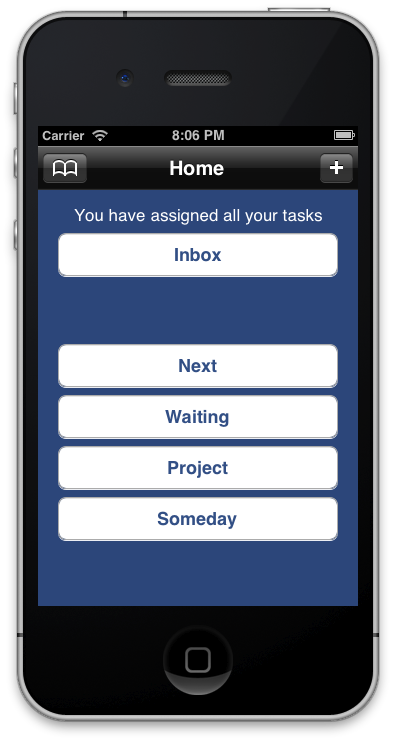
\includegraphics[height=12.5cm]{main.png}
	\caption{Vista de principal}
\end{figure}

A la hora de a\~nadir una nueva tarea nos encontramos ante una vista sencilla que nos presenta tres campos b\'asicos:

\begin{itemize}
	\item Nombre.
	\item Descripci\'on.
	\item Prioridad.
\end{itemize}

La categor\'ia que se le asignar\'a es Inbox autom\'aticamente siguiendo el esquema de funcionamiento de GTD, por lo que el usuario no debe preocuparse de escoger una categor\'ia en este punto. La fecha de creaci\'on tambi\'en es asignada autom\'aticamente por el programa.

\begin{figure}[h]
	\centering
	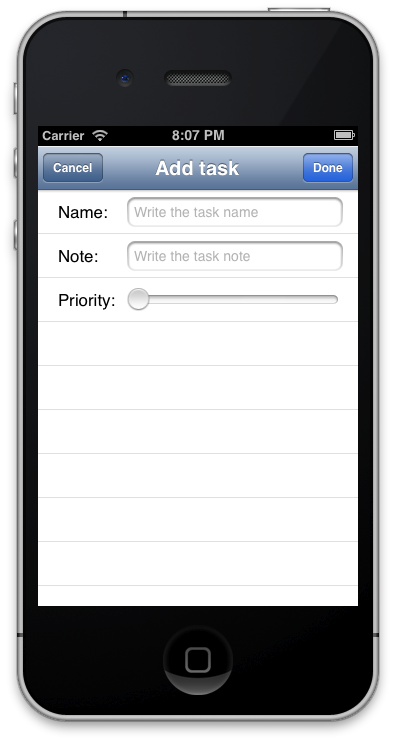
\includegraphics[height=12.5cm]{add.png}
	\caption{Nueva tarea}
\end{figure}

Como vemos esta vista est\'a enfocada a la rapidez y la sencillez, de forma que el proceso para crear una nueva tarea sea muy \'agil y permita al usuario despreocuparse de ella cuanto antes.

Una vez creada la tarea nos devolverá a la vista principal.

Si escogemos una categor\'ia pulsando sobre el bot\'on correspondiente desde la página de inicio nos mostrar\'a una lista de las tareas asociadas a dicha categor\'ia. Desde aqu\'i podremos seleccionar la tarea que queremos ver en m\'as detalle u ordenar la visualizaci\'on de las tareas siguiendo un criterio espec\'ifico pulsando sobre el icono que se encuentra en la parte derecha de la barra de navegaci\'on superior.

\begin{figure}[h]
	\centering
	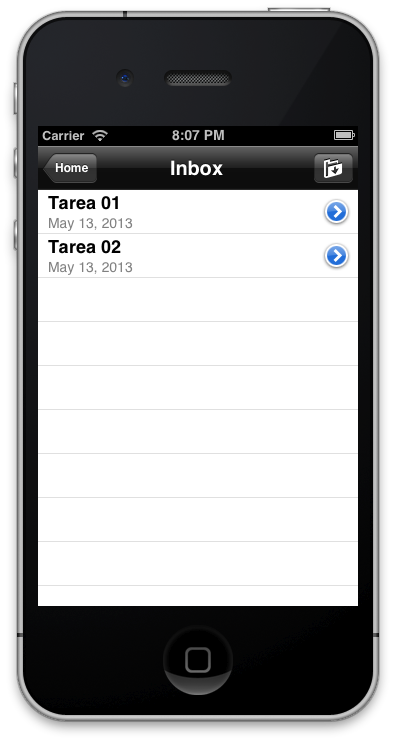
\includegraphics[height=12.5cm]{category.png}
	\caption{Vista de categoria}
\end{figure}

Para acceder a una vista en detalle de una tarea concreta solo hace falta pulsar sobre ella.

En esta vista más detallada sobre la tarea encontramos toda la informaci\'on relativa a esta, desde su nombre hasta su fecha de creaci\'on, as\'i como la categor\'ia a la que pertenece. Desde esta vista adem\'as se puede marcar la tarea como completada o borrarla usando los botones de la parte inferior.

Si queremos editar la tarea para modificar su informaci\'on o asignarle una categor\'ia distinta podemos hacerlo desde el bot\'on dispuesta en la parte superior derecha, que nos llevar\'a hasta una vista de edici\'on donde podremos cambiar la tarea como deseemos.

\begin{figure}[h]
	\centering
	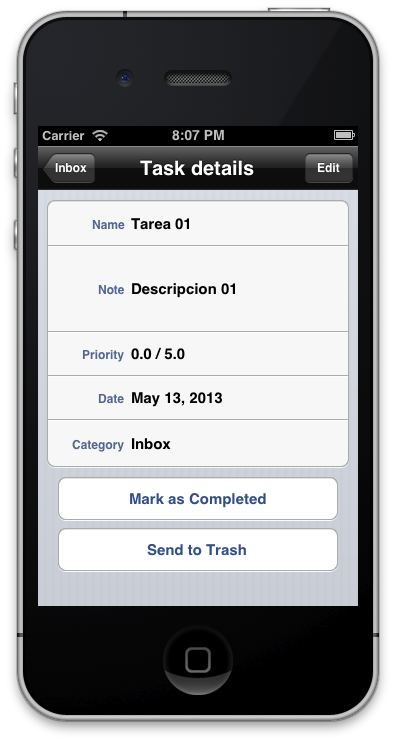
\includegraphics[height=10.5cm]{task.png}
	\caption{Vista de tarea}
\end{figure}


\end{document}